\documentclass[tikz,border=7pt]{standalone}
\begin{document}
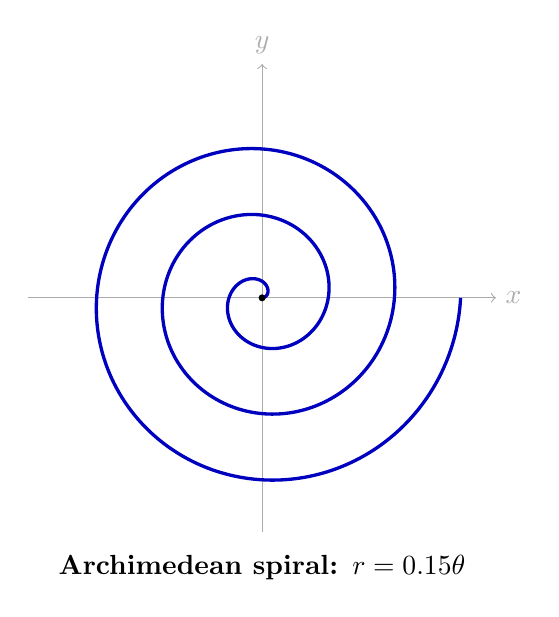
\begin{tikzpicture}[scale=.9]
\draw[->,gray!65] (-3.3,0)--(3.3,0) node[right] {$x$};
\draw[->,gray!65] (0,-3.3)--(0,3.3) node[above] {$y$};
\draw[blue!75!black,very thick,samples=520,domain=0:1080,smooth,variable=\t]
  plot ({.0026*\t*cos(\t)},{.0026*\t*sin(\t)});
\fill (0,0) circle (1.4pt);
\node[font=\bfseries] at (0,-3.8) {Archimedean spiral: $r=0.15\theta$};
\end{tikzpicture}
\end{document}
